% -*- LaTeX -*-
% -*- coding: utf-8 -*-
%
% michael a.g. aïvázis
% california institute of technology
% (c) 1998-2012 all rights reserved
%

\lecture{Introduction to \pyre}{20120516}

% --------------------------------------
% recap
\begin{frame}[fragile]
%
  \frametitle{Recap: what we know so far}
%
  \begin{itemize}
%
  \item \pyre\ components are evolved python objects
    \begin{itemize}
    \item the factories have family names, the instances have names
    \item these names are unique strings in hierarchical namespaces delimited by periods
    \item collections of components form packages \emph{implicitly}, based on the topmost level
      in their namespace
    \end{itemize}
%
  \item components have properties that are under the control of the \emph{user}
    \begin{itemize}
    \item they look and behave like regular attributes
    \item they are \emph{typed} to enable conversions from strings
    \item they have default values and other metadata
    \end{itemize}
%
  \item configuration is partly about assigning values to component properties
    \begin{itemize}
    \item a requirement for supporting user interfaces
    \item intuitive syntax for the command line
    \item simple configuration files inspired by the Microsoft Windows \identifier{.ini} format
    \end{itemize}
%
  \item configuration is automatically handled by the framework and requires no explicit
    involvement on the part of the component author
%
  \end{itemize}
%
\end{frame}

% --------------------------------------
% memory refresh
\begin{frame}[fragile]
%
  \frametitle{A simple component}
%
  \begin{ipython}{}
import pyre

class Disk(pyre.component, family="gauss.shapes.disk"):

    # public state
    radius = pyre.properties.float()
    radius.default = 1
    radius.doc = 'the radius of the disk'

    center = pyre.properties.array()
    center.default = (0,0)
    center.doc = 'the location of the center of the circle'

    # interface
    @pyre.export
    def interior(self, points):
        """
        Filter {points} by removing exterior ones
        """
        ...
  \end{ipython}
%
\end{frame}

% --------------------------------------
% a sample configuration
\begin{frame}[fragile]
%
  \frametitle{A simple configuration file}
%
  \begin{itemize}
%
  \item a file named \srcfile{gauss.cfg} with the following
%
  \begin{icfg}{}
 [ gauss.shapes.disk ] ; the family name
 radius = 2
 center = (-1,-1)

 [ disk1 ] ; the name of an instance
 center = (-1,1)   ; leave {radius} alone

 [ disk2 ] ; the name of another instance
 radius = .5
 center = (1,1)
  \end{icfg}
%
  could get loaded automatically when \component{Disk} is first imported, or loaded by naming it
  explicitly on the command line
%
  \item the \srcfile{.cfg} extension allows the framework to deduce which configuration file
    parser should be used to process the contents
%
  \end{itemize}
%
\end{frame}

% --------------------------------------
% explore
%\begin{frame}[fragile]
%
  %\frametitle{Interactive explorations}
%
%\end{frame}

% --------------------------------------
% template
\begin{frame}[fragile]
%
  \frametitle{Configuration files}
%
  \begin{itemize}
%
  \item currently, there are two file formats for configuration information
    \begin{itemize}
    \item \srcfile{.cfg}: the format in the examples
    \item \srcfile{.pml}: an \srcfile{XML} based format that is a bit more powerful but not as
      user friendly
    \end{itemize}
%
  \item \pyre\ looks for configuration files in the following places
    \begin{itemize}
    \item explicitly provided on the command line
      \begin{ish}{}
 gauss.py --config=sample.cfg
      \end{ish}
    \item the current directory
    \item the \srcfile{.pyre} subdirectory of the current user's home directory
    \item a special subdirectory wherever \pyre\ is installed
    \end{itemize}
    in order of priority
%
  \item settings on the command line have the highest priority, and override each other from
    left to right
%
  \item when a property is assigned a value multiple times, the highest priority setting wins
    \begin{itemize}
    \item the framework keeps track of all changes in the value of properties and the source of
      the assignment, so if a property doesn't end up with the value you expected, you can get
      its complete history
    \end{itemize}
%
  \end{itemize}
%
\end{frame}

% --------------------------------------
% properties
\begin{frame}[fragile]
%
  \frametitle{Properties}
%
  \begin{itemize}
%
  \item properties make sense for both classes and instances
    \begin{itemize}
    \item the class holds the default value that gets used in case the component instance does
      not have explicit configuration
    \item each instance gets its own private value when it gets configured
    \item identical to regular python attributes
    \end{itemize}
%
  \item there is support for 
    \begin{itemize}
    \item simple types: \function{bool}, \function{int}, \function{float}, \function{str}
    \item containers: \function{tuple}, \function{array}
    \item higher level: \function{date}, \function{time}, \function{inputfile},
      \function{outputfile}, \function{inet}
    \item units: \function{dimensional}
    \item easy enough to implement your own; the requirements are very simple
    \end{itemize}
%
  \item metadata:
    \begin{itemize}
    \item \identifier{doc}: a simple and short documentation string
    \item \identifier{default}: the default value, in case the user doesn't supply one
    \item \identifier{converters}: a chain of preprocessors of the string representation
    \item \identifier{normalizers}: a chain of post-processors of the converted value
    \item \identifier{validators}: a tuple of predicates that get called to ensure the property
      value satisfies the specified constraints
    \item you can add your own; the framework passes them through to your component
    \end{itemize}
%
  \end{itemize}
%
\end{frame}

% --------------------------------------
% units
\begin{frame}[fragile]
%
  \frametitle{Units}
%
  \begin{itemize}
%
  \item \function{dimensional} properties have units
%
  \item the low level support is in \package{pyre.units}
    \begin{itemize}
    \item full support for all SI base and derived units
    \item all common abbreviations and names from alternative systems of units
    \item correct arithmetic; proper handling of functions from \package{math}
    \end{itemize}
%
    \begin{ipython}{}
from math import cos
from pyre.units.SI import meter, second, radian

A = 2.5 * meter
t = 1.5 * second
#@$\omega$@ = 4.2 * radian/second

x = A * cos(#@$\omega$@ * t)
    \end{ipython}
%
    if the units in the argument to \function{cos} do not cancel, leaving a pure
    \keyword{float} behind, an exception is raised; \identifier{x} has dimensions of meters
%
  \end{itemize}
%
\end{frame}

% --------------------------------------
% facilities
\begin{frame}[fragile]
%
  \frametitle{Connecting components}
%
  the real power is in wiring components to other components
%
  \begin{ipython}{}
import pyre

class MonteCarlo(pyre.component, family="gauss.integrators.montecarlo"):
    """
    A Monte Carlo integrator
    """

    # public state
    samples = pyre.property.int(default=10**5)
    region = ????
    ...
  \end{ipython}
%
  \begin{itemize}
  \item \component{MonteCarlo} should be able to specify what constitutes an acceptable region
  \item \component{Disk} should be able to advertise itself as being an acceptable
    region
  \item the user should have natural means for specifying that she wants to wire an instance of
    \component{Disk} as the region of integration
  \item and be able to configure that particular instance of \component{Disk} in a natural
    manner
  \item the framework should check the consistency of this assignment
  \end{itemize}
%
\end{frame}

% --------------------------------------
% interfaces
\begin{frame}[fragile]
%
  \frametitle{Interfaces}
%
  the component version of our abstract base class is the \emph{interface}
%
  \begin{ipython}[basicstyle=\tt\tiny]{}
import pyre

class Shape(pyre.interface, family="gauss.shapes"):
    """
    The obligations of implementations of geometrical shapes
    """

    # my default implementation
    @classmethod
    def default(cls):
        """
        The default {Shape} implementation
        """
        # use a box
        from .Box import Box
        return Box # if you return an instance, it will be shared by all...

    # interface
    @pyre.provides
    def measure(self):
        """
        Compute my measure: length, area, volume, etc
        """
        
    @pyre.provides
    def interior(self, points):
        """
        Filter out {points} that are on my exterior
        """
  \end{ipython}
%
  \pyre\ prohibits the instantiation of interfaces, so you don't have to worry about the
  implementation of the methods
%
\end{frame}

% --------------------------------------
% disk revisited
\begin{frame}[fragile]
%
  \frametitle{Declaring compatibility with an interface}
%
  \component{Disk} can inform the framework that it intends to implement \interface{Shape}
%
  \begin{ipython}{}
import pyre
from Shape import Shape

class Disk(pyre.component, family="gauss.shapes.disk", implements=Shape):
    """
    A representation of a circular disk
    """

    ...
  \end{ipython}
%
  an exception is raised if \component{Disk} does not conform fully to \interface{Shape}
%
  \begin{itemize}
  \item missing methods or missing attributes
  \end{itemize}
%
  also, proper namespace design simplifies many things for the user
%
  \begin{itemize}
  \item \interface{Shape} declared its family as \identifier{gauss.shapes}
  \item \component{Disk} declared its family as \identifier{gauss.shapes.disk}
  \end{itemize}
%
  we'll see how later when it's time to put all this together
%
\end{frame}

% --------------------------------------
% facilities
\begin{frame}[fragile]
%
  \frametitle{Specifying assignment requirements}
%
  \component{MonteCarlo} can now specify it expects a \interface{Shape} compatible object to be
  assigned as its region of integration
%
  \begin{ipython}{}
import pyre
from Shape import Shape

class MonteCarlo(pyre.component, family="gauss.integrators.montecarlo"):
    """
    A Monte Carlo integrator
    """

    # public state
    samples = pyre.property.int(default=10**5)
    region = pyre.facility(interface=Shape)
    ...
  \end{ipython}
%
  the default value is whatever \interface{Shape} returns from its \function{default} class
  method
%
\end{frame}

% --------------------------------------
% component specification
\begin{frame}[fragile]
%
  \frametitle{Component specification}
%
  \begin{itemize}
%
  \item and now for the real trick: converting some string provided by the user into a live
    instance of \component{Disk}, configuring it, and attaching it to some
    \component{MonteCarlo} instance
%
  \item the syntax is motivated by \identifier{URI}, the universal resource identifiers of the
    web; the general form is
    \begin{icfg}{}
      <scheme>://<authority>/<path>#<identifier>
    \end{icfg}
    where most of the segments are optional
%
  \item if your component is accessible from your python path, you could specify
    \begin{icfg}{}
      import:gauss.shapes.disk
    \end{icfg}
%
  \item if your component instance is somewhere on your disk, you would specify
    \begin{icfg}{}
      file:/tmp/shapes.py/disk
    \end{icfg}
%
  \item in either case, \function{disk} is expected to be a name that resolves into a component
    class, a component instance or be a callable that returns one of these
%
  \end{itemize}
%
\end{frame}

% --------------------------------------
% the user does the wiring
\begin{frame}[fragile]
%
  \frametitle{The user does the wiring}
%
  with our definition of \component{MonteCarlo}, an appropriately structured package
  \package{gauss} on the python path, and the following configuration file
%
  \begin{icfg}{}
 [ gauss.shapes.disk ] ; change the default values for all disks
 radius = 1
 center = (0,0)

 [ mc ] ; configure our Monte Carlo integrator instance
 region = import:gauss.shapes.disk
 ...
  \end{icfg}{}
%
 the following python code in some script \srcfile{sample.py}
%
 \begin{ipython}{}
   ...
   mc = MonteCarlo(name="mc")
   ...
 \end{ipython}
%
 builds a \component{MonteCarlo} instance and configures it so that its region of
 integration is a \component{Disk} instance; similarly, from the command line
%
 \begin{ish}{}
    sample.py --mc.region=import:gauss.shapes.disk
 \end{ish}
%
 or, thanks to the consistency in our namespace layout, simply
%
 \begin{ish}{}
    sample.py --mc.region=disk
 \end{ish}
%
\end{frame}

% --------------------------------------
% namespace design
\begin{frame}[fragile]
%
  \frametitle{Namespace design}
%
  we are now in a position to assemble the package \package{gauss}; let's start by laying out
  the package namespace
%
  \begin{figure}
    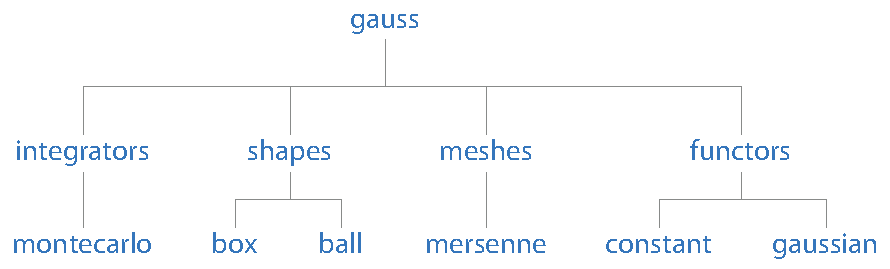
\includegraphics[scale=0.5]{figures/gauss-namespace.pdf}
  \end{figure}
%
  and let's try to use this layout for both the logical and physical structure
  \begin{itemize}
  \item the top level is our package name
  \item the internal nodes become the names of interfaces and subdirectories
  \item the leaves are the component family names and the names by which the component
    factories are accessible
  \end{itemize}
%
\end{frame}
% end of file 
